\documentclass[11pt,twocolumn,a4paper]{article}

\usepackage{amsmath,amssymb,amsthm}
\usepackage{mathtools}
\usepackage{natbib}
\usepackage{hyperref}
\usepackage{cleveref}
\usepackage{geometry}
\usepackage{enumitem}
\usepackage{xcolor}
\usepackage{booktabs}
\usepackage{array}
\usepackage{microtype}
\usepackage{graphicx}
\graphicspath{{figures/}}
\geometry{top=2.2cm, bottom=2.5cm, left=2.0cm, right=2.0cm, columnsep=0.7cm}

%% Theorem environments
\theoremstyle{plain}
\newtheorem{theorem}{Theorem}[section]
\newtheorem{lemma}[theorem]{Lemma}
\newtheorem{proposition}[theorem]{Proposition}
\newtheorem{corollary}[theorem]{Corollary}
\theoremstyle{definition}
\newtheorem{definition}[theorem]{Definition}
\newtheorem{assumption}[theorem]{Assumption}
\newtheorem{example}[theorem]{Example}
\theoremstyle{remark}
\newtheorem{remark}[theorem]{Remark}

%% Notation macros
\newcommand{\N}{\mathcal{N}}
\newcommand{\E}{\mathcal{E}}
\newcommand{\T}{\mathcal{T}}
\newcommand{\X}{\mathcal{X}}
\newcommand{\G}{\mathcal{G}}
\renewcommand{\H}{\mathcal{H}}
\newcommand{\B}{\mathcal{B}}
\newcommand{\C}{\mathcal{C}}
\newcommand{\F}{\mathcal{F}}
\newcommand{\R}{\mathbb{R}}
\newcommand{\Z}{\mathbb{Z}}
\newcommand{\tick}{\tau_0}
\newcommand{\sep}{\mathrm{sep}}
\newcommand{\yield}{\mathrm{yield}}
\newcommand{\floor}{\beta}
\newcommand{\dcat}{d_{\mathrm{cat}}}
\newcommand{\norm}[1]{\left\|#1\right\|}
\newcommand{\abs}[1]{\left|#1\right|}
\newcommand{\cell}{\mathrm{cell}}
\newcommand{\Scal}{S}
\newcommand{\Lyap}{V}
\newcommand{\kap}{\kappa}
\newcommand{\pres}{P}
\DeclareMathOperator*{\argmax}{arg\,max}
\DeclareMathOperator*{\argmin}{arg\,min}

\title{\textbf{Network Yield and Computing Allocation:\\
A Unified Framework for Distributed Task Scheduling\\
via Thermodynamic Resolution Floors, Cell-Partition Control,\\
and Market Clearing}}

\author{Kundai Farai Sachikonye\\[2pt]
\small Technical University Muenchen\\
\small AIMe Registry for Artificial Intelligence\\
\small \texttt{kundai.sachikonye@wzw.tum.de}}
\date{\today}



\begin{document}

\maketitle

\begin{abstract}
We develop a self-contained theory of distributed computing allocation in which every schedulable resource, every state observation, and every economic signal shares a single irreducible quantum $\tick > 0$: the \emph{compute-tick}. The framework rests on three foundations assembled into a unified object. First, a \emph{finite observer axiom} forces every monitor to return a cell rather than a point, establishing a resolution floor $\floor \geq \tick > 0$ that bounds observation precision absolutely. Second, a \emph{cell-partition scheduler} compiled from offline stability analysis governs task placement with a Lyapunov guarantee and a Banach contraction whose ratio is computable without runtime measurement. Third, a \emph{separation-cost functional} assigns to every execution slot a yield price equal to its marginal contribution to useful task progress, and the clearing map for those prices coincides with the yield-optimal assignment and with deterministic scheduler closure at the same fixed point.

The central result is a \emph{Three-way Equivalence}: yield-optimality, deterministic closure, and market clearing are one fixed point, coinciding because $\tick$ serves simultaneously as the physical resolution floor for observations, the algorithmic closure threshold for the scheduler, and the minimum lot size for the clearing market. From this equivalence we derive, as theorems rather than assumptions, that executor threads run at forced slot-optimal utilisation ratios, that tasks sort onto execution slots by comparative advantage in compute-ticks, and that a purely local, residual-work-descent routing law drains every task queue in finite time because the separation cost raised by a stalled queue is identical to the yield signal that summons an executor. A structural incorruptibility theorem guarantees that no monitoring payload can influence the scheduling action stream without traversing an explicit approval boundary. Finally, we invert the locus of agency: an allocated process is re-read as a \emph{persistent goal-directed agent} that pursues its own target every tick, succeeds to a fresh goal on completion rather than terminating, returns a distinct response on each interaction because its inner state has advanced, and summons capacity by raising its own price when stalled---each of these properties a theorem of the same machinery, with goal succession the one added primitive. All proofs are given in full; no prior companion paper is required.
\end{abstract}

\tableofcontents

%% ===================================================================
\section{Introduction}
\label{sec:intro}
%% ===================================================================

Distributed computing systems schedule tasks onto processors, manage queues of pending work, observe system state, and route tasks between machines. Despite decades of theory---backpressure scheduling \cite{tassiulas1992}, fluid models \cite{neely2010}, fair queueing \cite{demers1990}, cluster managers \cite{hindman2011,verma2015}---no unified account explains simultaneously why a correct scheduler \emph{cannot} observe state with arbitrary precision, why the scheduler that maximises useful throughput is the same one that clears a natural market, and why both coincide with the fixed point of a pure local rule requiring no global coordination.

This paper provides that account. The central object is a \emph{computing network} $\G = (\N, \E)$: a finite set of \emph{queue nodes} $\N$ (buffers for pending tasks) and a finite set of \emph{execution slots} $\E$ (processors), each with a capacity and a cost. Tasks carry private completion targets; the objective is useful target-ward progress per unit compute-tick. The key insight is that a single positive quantum $\tick > 0$---the minimum schedulable unit of processor time---appears in three distinct roles:
\begin{itemize}[nosep]
\item \emph{Physical}: the resolution floor below which no monitor can distinguish system states;
\item \emph{Algorithmic}: the gap below which the scheduler cannot improve by reassigning a single task;
\item \emph{Economic}: the minimum lot size in the clearing market for execution capacity.
\end{itemize}

When these three roles are played by the same $\tick$, the three fixed-point conditions coincide and the Three-way Equivalence holds. When the roles are played by distinct constants, the equivalence degrades gracefully: the slack grows to the maximum of the three constants and the clearing price deviates from the separation cost by the algorithmic-economic split.

\paragraph{Organisation.} Section~\ref{sec:model} defines the computing network model and all primitive objects. Section~\ref{sec:floor} establishes the resolution floor theorem. Section~\ref{sec:monitor} develops the monitoring architecture: S-entropy state space, trajectory completion operator, and the monitor--control separation theorem. Section~\ref{sec:scheduler} presents the cell-partition scheduler with its stability and contraction theorems. Section~\ref{sec:separation} defines separation costs and the yield functional. Section~\ref{sec:equivalence} proves the Three-way Equivalence. Section~\ref{sec:liveness} proves liveness under backpressure coupling. Section~\ref{sec:incorruptibility} proves structural incorruptibility. Section~\ref{sec:agents} inverts the locus of agency, recasting allocated processes as persistent goal-directed agents and adding the goal-succession primitive. Section~\ref{sec:discussion} situates the results in the literature. Section~\ref{sec:conclusion} concludes.

\paragraph{Prerequisites.} The paper is self-contained. Familiarity with basic real analysis (metric spaces, fixed-point theorems) and linear algebra (eigenvalues, positive-definite matrices) suffices.

%% ===================================================================
\section{The Computing Network Model}
\label{sec:model}
%% ===================================================================

\subsection{Primitive objects}

\begin{definition}[Computing network]
\label{def:network}
A \emph{computing network} is a tuple $\G = (\N, \E, c, \ell, \bar{v})$ where:
\begin{itemize}[nosep]
\item $\N = \{n_1, \ldots, n_K\}$ is a finite set of \emph{queue nodes} (buffers);
\item $\E = \{e_1, \ldots, e_M\}$ is a finite set of \emph{execution slots} (processors);
\item $c : \E \to \mathbb{Z}_{>0}$ assigns each slot a \emph{thread capacity} $c(e) \geq 1$;
\item $\ell : \E \to \R_{>0}$ assigns each slot an \emph{expected task duration} $\ell(e) > 0$;
\item $\bar{v} : \E \to \R_{>0}$ assigns each slot a \emph{maximum throughput rate} $\bar{v}(e) > 0$.
\end{itemize}
\end{definition}

\begin{definition}[Compute-tick]
\label{def:tick}
The \emph{compute-tick} $\tick > 0$ is the minimum indivisible unit of processor time. No scheduling decision, observation, or price can be expressed to a precision finer than $\tick$.
\end{definition}

\begin{remark}
In practice $\tick$ corresponds to the OS scheduler quantum, the minimum time-slice allocated by the kernel. Its existence is not an engineering choice but a consequence of the finite-observer axiom proved in Section~\ref{sec:floor}.
\end{remark}

\begin{definition}[Task]
\label{def:task}
A \emph{task} $x$ is a tuple $(o(x), \tau(x), w(x))$ where $o(x) \in \N$ is the \emph{originating queue node}, $\tau(x) \in \R^d$ is the \emph{completion target} (a feature vector encoding the desired output state), and $w(x) > 0$ is the \emph{work estimate} (expected compute-ticks to completion).
\end{definition}

\begin{definition}[Residual work]
\label{def:residual}
For a task $x$ currently executing on slot $e$, the \emph{residual work} is
\[
  r(x, e) \;=\; \rho\bigl(\mathrm{loc}(x),\; \tau(x)\bigr),
\]
where $\mathrm{loc}(x) \in \R^d$ is the current state of $x$'s computation (the partial result produced so far) and $\rho$ is the Euclidean distance on $\R^d$.
\end{definition}

\begin{definition}[Queue occupancy and directional pressure]
\label{def:pressure}
Let $\X(n)$ denote the set of tasks currently queued at node $n \in \N$, and let $\mathrm{hd}(e) \in \R^d$ denote the ``head'' of slot $e$: the state at which a task assigned to $e$ arrives after one tick of execution. The \emph{directional pressure} from node $n$ towards slot $e$ is
\[
  \pres(n, e) \;=\; \sum_{x \in \X(n)} \bigl[r(x, e) - \rho(\mathrm{hd}(e), \tau(x))\bigr]^{+},
\]
where $[z]^+ = \max(z, 0)$. Tasks that would \emph{not} make progress by moving to $e$ contribute zero pressure.
\end{definition}

\begin{definition}[Network transport yield]
\label{def:yield}
The \emph{network transport yield} of an assignment $A : \X \to \E$ (a map from tasks to slots) is
\[
  \yield(A) \;=\; \frac{\displaystyle\sum_{x \in \X} \bigl[r(x, A(x)) - \rho(\mathrm{hd}(A(x)), \tau(x))\bigr]^{+}}
                        {\displaystyle\sum_{e \in \E} \tick \cdot c(e) \cdot g_u(v(e))},
\]
where $v(e) \in (0, \bar{v}(e)]$ is the throughput rate at which slot $e$ operates under assignment $A$, and $g_u : \R_{>0} \to \R_{>0}$ is a strictly convex \emph{utilisation cost} satisfying $g_u' > 0$ and $g_u'' > 0$.

\noindent
The numerator counts total target-ward progress; the denominator counts total resource consumption in compute-ticks weighted by utilisation cost.
\end{definition}

\subsection{Separation cost}

\begin{definition}[Separation cost]
\label{def:sep}
The \emph{separation cost} of slot $e$ under assignment $A$ is the marginal yield lost by removing $e$ from the network:
\[
  \sep(e, A) \;=\; \yield(A) \;-\; \yield(A|_{\E \setminus \{e\}}),
\]
where $A|_{\E \setminus \{e\}}$ is the optimal re-assignment of tasks after removing $e$.
\end{definition}

\begin{remark}
$\sep(e, A) \geq 0$. A redundant slot ($e$ has a perfect substitute) has $\sep = 0$; a bottleneck slot has large $\sep$.
\end{remark}

\subsection{Assignments and closure}

\begin{definition}[Single-slot reassignment neighbourhood]
\label{def:neighborhood}
Two assignments $A$ and $A'$ are \emph{$\tick$-adjacent} if they differ in the allocation of at most one task and the resulting change in yield is at most $\tick$.
\end{definition}

\begin{definition}[Deterministic closure]
\label{def:closure}
Assignment $A$ is \emph{deterministically closed} if no $\tick$-adjacent assignment $A'$ satisfies $\yield(A') > \yield(A) + \tick$. Equivalently, the best single-task reassignment cannot improve yield beyond the resolution floor.
\end{definition}

%% ===================================================================
\section{The Resolution Floor}
\label{sec:floor}
%% ===================================================================

\subsection{Finite observer axiom}

\begin{assumption}[Finite observer]
\label{ass:finite}
Any monitoring subsystem of the computing network is itself a finite computational process: it runs on hardware with a finite number of distinguishable states, communicates over channels with finite bandwidth, and terminates its observation procedure in finite time.
\end{assumption}

This axiom is not a limitation of current technology; it is a logical consequence of a bounded physical substrate. It implies the following foundational theorem.

\begin{theorem}[Resolution floor]
\label{thm:floor}
Under Assumption~\ref{ass:finite}, there exists $\floor > 0$ such that for every observable quantity $q$ and every monitor $\mathcal{M}$, the identification $\mathcal{M}(q)$ satisfies
\[
  \inf_q \;\mathrm{diam}\bigl(\mathcal{M}(q)\bigr) \;\geq\; \floor \;>\; 0,
\]
where $\mathrm{diam}(\cdot)$ is the diameter of the set $\mathcal{M}(q) \subseteq \R$ returned by $\mathcal{M}$.

No monitor returns a point; every identification carries strictly positive irreducible residual uncertainty.
\end{theorem}

\begin{proof}
Let $S$ be the finite state space of $\mathcal{M}$ and let $Q$ be the range of $q$. $\mathcal{M}$ defines a function $f : Q \to 2^Q$. Since $S$ is finite, $f$ has at most $|S|$ distinct outputs. The pre-images $\{f^{-1}(r) : r \in \mathrm{range}(f)\}$ partition $Q$ into at most $|S|$ cells. Since $Q$ is a metric space with at least $|S|+1$ distinct points (for any finite $S$, the range of a physical quantity is infinite in principle), at least one cell has diameter $\geq \mathrm{diam}(Q)/|S| > 0$. Setting $\floor = \min_{r} \mathrm{diam}(f^{-1}(r))$ and noting that every cell must have positive diameter (because $q$ is a continuous physical quantity) gives $\floor > 0$.

Formally: suppose for contradiction that some cell $f^{-1}(r)$ has diameter zero. Then $f^{-1}(r)$ is a single point, and $f$ distinguishes that point from all others---which requires $|S| \geq |Q|$. But $Q$ is uncountable (it is a real-valued quantity) and $S$ is finite, a contradiction.
\end{proof}

\begin{corollary}[Compute-tick as floor]
\label{cor:tick_floor}
The compute-tick $\tick$ satisfies $\tick \geq \floor$. Scheduling decisions made at resolution $\tick$ are consistent with the observation resolution guaranteed by Theorem~\ref{thm:floor}.
\end{corollary}

\begin{proof}
Any scheduling decision that distinguishes two system states separated by less than $\floor$ would require a monitor that violates Theorem~\ref{thm:floor}. Therefore, the minimum indivisible decision granularity must be $\geq \floor$. Setting $\tick = \floor$ achieves the tightest consistent granularity.
\end{proof}

%% ===================================================================
\section{Monitoring Architecture}
\label{sec:monitor}
%% ===================================================================

\subsection{S-entropy state space}

\begin{definition}[S-normalisation]
\label{def:snorm}
For a physical quantity $q$ with known bounds $[q_{\min}, q_{\max}]$, the \emph{S-normalisation} is
\[
  \Scal(q) \;=\; \frac{q - q_{\min}}{q_{\max} - q_{\min}} \;\in\; [0,1].
\]
S-normalisation maps heterogeneous dimensional quantities onto a common unit interval, enabling uniform treatment of queue lengths, utilisation rates, task progress fractions, and thermal metrics.
\end{definition}

\begin{definition}[S-entropy state space]
\label{def:sspace}
Let the observable state of the computing network be described by $m$ independent quantities $q_1, \ldots, q_m$. The \emph{S-entropy state space} is
\[
  \H \;=\; [0,1]^m,
\]
equipped with the Euclidean metric. Each coordinate $\Scal(q_i)$ represents one observable dimension. $\H$ is compact, connected, and a complete metric space.
\end{definition}

\begin{remark}
The three canonical coordinates are: $s_k = \Scal(\text{queue occupancy})$ (knowledge entropy), $s_t = \Scal(\text{task age})$ (temporal entropy), and $s_e = \Scal(\text{residual work fraction})$ (evolution entropy). Additional coordinates may encode thermal load, network latency, and memory pressure.
\end{remark}

\subsection{Cell partition and the monitoring cell}

\begin{definition}[Cell partition]
\label{def:cellpartition}
A \emph{cell partition} $\C = \{C_1, \ldots, C_N\}$ is a finite Borel partition of $\H$ such that each cell $C_i$ has width $w_i \geq \floor > 0$.
\end{definition}

\begin{definition}[Monitoring cell]
\label{def:moncell}
For an observed state $h \in \H$, the \emph{monitoring cell} is the unique $C_i \in \C$ containing $h$:
\[
  \cell(h) \;=\; C_i \quad \Leftrightarrow \quad h \in C_i.
\]
The monitor returns $\cell(h)$, not $h$ itself. This is consistent with Theorem~\ref{thm:floor}: the cell has diameter $\geq \floor > 0$.
\end{definition}

\subsection{Trajectory completion}

Computing networks exhibit partially observable dynamics: a task's computational trajectory from initiation to completion is not directly accessible but must be inferred from snapshots of residual work.

\begin{definition}[Fuzzy network state]
\label{def:fuzzy}
A \emph{fuzzy network state} is a function $\mu : \N \times \E \to [0,1]$ assigning to each (queue-node, slot) pair a belief weight, with $\sum_{n,e} \mu(n,e) = 1$.
\end{definition}

\begin{definition}[State space of fuzzy states]
\label{def:fuzzyspace}
Let $\F$ be the set of all fuzzy network states. Equipped with the $\ell^1$ metric $d_1(\mu, \nu) = \sum_{n,e} |\mu(n,e) - \nu(n,e)|$, $(\F, d_1)$ is a complete metric space.
\end{definition}

\begin{definition}[Trajectory completion operator]
\label{def:trajop}
Define the \emph{trajectory completion operator} $\T = \T_{\mathrm{kin}} \circ \T_{\mathrm{therm}} \circ \T_{\mathrm{bal}}$ on $\F$:
\begin{itemize}[nosep]
\item $\T_{\mathrm{bal}}$ rebalances belief weights to be consistent with observed queue occupancies;
\item $\T_{\mathrm{therm}}$ applies a diffusion step consistent with the maximum-entropy principle over unobserved paths;
\item $\T_{\mathrm{kin}}$ projects forward by one tick using the assignment kinematics.
\end{itemize}
\end{definition}

\begin{theorem}[Trajectory completion converges]
\label{thm:traj}
Under Assumption~\ref{ass:finite} and with a fixed assignment $A$, the operator $\T$ is a Banach contraction on $(\F, d_1)$ with contraction ratio $\rho_{\T} < 1$. In particular, there exists a unique fixed point $\mu^* \in \F$ with $\T(\mu^*) = \mu^*$, and for any initial $\mu_0 \in \F$,
\[
  d_1\bigl(\T^k(\mu_0),\; \mu^*\bigr) \;\leq\; \rho_{\T}^k \cdot d_1(\mu_0, \mu^*),
\]
so the sequence $(\T^k(\mu_0))$ converges geometrically to $\mu^*$.
\end{theorem}

\begin{proof}
$\T_{\mathrm{bal}}$ is a projection onto the closed convex set of distributions consistent with observations; as a nearest-point projection in $\ell^1$ onto a convex set, it is non-expansive. $\T_{\mathrm{therm}}$ applies a strictly positive stochastic matrix $Q$ (the maximum-entropy diffusion kernel); by the Perron--Frobenius theorem, $Q$ has a unique stationary distribution and its spectral gap is $1 - \lambda_2(Q) > 0$, so multiplication by $Q$ is a contraction in $\ell^1$ with ratio $\leq 1 - \text{gap}(Q) < 1$. $\T_{\mathrm{kin}}$ is a deterministic permutation of the state; it is an isometry, hence non-expansive. The composition of a strict contraction with non-expansive maps is a strict contraction \cite{banach1922}. Setting $\rho_{\T} = 1 - \text{gap}(Q) < 1$ completes the proof.
\end{proof}

\subsection{Closure dichotomy for monitoring}

\begin{definition}[Monitoring confirmation]
\label{def:confirm}
A monitoring process over a finite set of sources $\Gamma = \{\gamma_1, \ldots, \gamma_n\}$ terminates in one of two states: \emph{confirmed} (sufficient evidence accumulated) or \emph{declined} (insufficient evidence; action withheld).
\end{definition}

\begin{theorem}[Confirm-or-decline dichotomy]
\label{thm:dichotomy}
Every monitoring process over finitely many sources with the closure criterion (Definition~\ref{def:closure} adapted to monitoring: no additional evidence reduces cell diameter below $\floor$) terminates in confirmed or declined. There is no third outcome.
\end{theorem}

\begin{proof}
The monitoring process accumulates evidence $e_1, e_2, \ldots$ from $n$ finite sources. By Assumption~\ref{ass:finite}, each source is a finite-state machine; the Cartesian product of $n$ finite-state machines is finite. The process therefore explores a finite directed graph of evidence states. Under the closure criterion, the process halts when no new transition reduces the diameter of the identified cell below $\floor$. Since the graph is finite, the process must reach a terminal state in finite steps. Terminal states partition into: states where the current cell meets the confirmation threshold (confirmed) and states where it does not (declined). There is no cycle that avoids both (the acyclicity follows from the requirement that each step must either reduce diameter or contribute new evidence; in a finite graph this eventually exhausts).
\end{proof}

\subsection{Coherence and sensor federation}

\begin{definition}[Mutually supporting cycle]
\label{def:cycle}
A set of monitoring sources $\{\gamma_1, \ldots, \gamma_n\}$ forms a \emph{mutually supporting cycle} if for each $i$, source $\gamma_i$ can confirm the output of $\gamma_{i-1 \bmod n}$ independently of all other sources.
\end{definition}

\begin{theorem}[Coherence requires three]
\label{thm:coherence}
A monitoring system is resilient to the arbitrary failure of any single source if and only if the remaining sources form a mutually supporting cycle of length $\geq 3$.
\end{theorem}

\begin{proof}
\emph{Necessity.} If all cycles in the dependency graph have length $\leq 2$, then every pair of sources supports only each other. Removing either element of such a pair destroys all support for the other, so the system is not resilient to single-source failure.

\emph{Sufficiency.} Suppose there exists a cycle $\gamma_1, \ldots, \gamma_n$ with $n \geq 3$. Remove source $\gamma_j$ for any $j$. The remaining cycle $\gamma_1, \ldots, \gamma_{j-1}, \gamma_{j+1}, \ldots, \gamma_n$ still has length $n-1 \geq 2$. For $n \geq 3$, $n - 1 \geq 2$ and the cycle is non-trivial. By the definition of mutual support, $\gamma_{j-1}$ is supported by $\gamma_{j-2}$ and $\gamma_{j+1}$ is supported by $\gamma_{j+2}$; the chain remains intact. Monitoring evidence can still propagate around the cycle, and the confirm-or-decline dichotomy (Theorem~\ref{thm:dichotomy}) is preserved.
\end{proof}

\begin{definition}[Multiplicative confirmation composition]
\label{def:multconf}
For independent confirmation sources $\gamma_1, \ldots, \gamma_n$ each with confirmation strength $\kap_i \in [0,1]$, the \emph{composite confirmation strength} is
\[
  \kap(\gamma_1 \circ \cdots \circ \gamma_n) \;=\; 1 - \prod_{i=1}^n (1 - \kap_i).
\]
\end{definition}

\subsection{Monitor--control separation theorem}

\begin{theorem}[Monitor--control separation]
\label{thm:separation}
A subsystem that acts on its own observations cannot simultaneously serve as an unbiased monitor of the system it controls.

Formally: let $\mathcal{M}$ be a monitor and $\mathcal{C}$ be a controller for the same system $\Sigma$. If $\mathcal{C}$'s actions are a function of $\mathcal{M}$'s outputs, then $\mathcal{M}$'s outputs are not independent of $\mathcal{C}$'s actions. In particular, any $\tick$-precise action by $\mathcal{C}$ induces a selection bias in $\mathcal{M}$ of at least $\floor$, violating the unbiasedness condition.
\end{theorem}

\begin{proof}
Let $h \in \H$ be the true system state. $\mathcal{M}$ returns $\cell(h)$ (Def.~\ref{def:moncell}). $\mathcal{C}$ reads $\cell(h)$ and executes action $u = A(\cell(h))$. The action $u$ modifies $\Sigma$ and therefore $h$: the post-action state is $h' = f(h, u)$ for some dynamics $f$. If $\mathcal{M}$ subsequently observes $h'$ to inform the same control cycle, its next output $\cell(h')$ depends on $u$, hence on $\cell(h)$, hence on the previous output of $\mathcal{M}$. The observation is therefore conditioned on the action, not independent of it.

For unbiasedness to hold, the monitor's output distribution must have conditional expectation $\mathbb{E}[\cell(h) | u] = \mathbb{E}[\cell(h)]$ for all $u$. But $u = A(\cell(h))$ makes $u$ a deterministic function of $\cell(h)$, so $h' = f(h, A(\cell(h)))$; the expectation $\mathbb{E}[\cell(h') | \cell(h)]$ is a non-trivial conditional distribution, not the marginal. The selection bias is the KL divergence between the conditional and marginal; since $\cell$ has diameter $\geq \floor > 0$ and $A$ maps distinct cells to distinct actions (by the schedulability condition), this divergence is at least $\log(1 + \floor / w_{\min}) > 0$, where $w_{\min}$ is the minimum cell width.

Therefore, monitoring and control must be separate processes whose outputs are never in the same feedback loop within one sampling period.
\end{proof}

%% ===================================================================
\section{Cell-Partition Scheduler}
\label{sec:scheduler}
%% ===================================================================

\subsection{Offline compilation}

The cell-partition scheduler pre-computes a lookup table $A : \C \to \E^{\X}$ mapping each monitoring cell to a task-to-slot assignment. This computation is performed offline; at runtime the scheduler reads the monitoring cell and performs a single table lookup.

\begin{definition}[Cell-partition scheduler]
\label{def:scheduler}
The \emph{cell-partition scheduler} is the function
\[
  u(t) \;=\; A\bigl(\cell(\Scal(h(t)))\bigr),
\]
where $h(t)$ is the observed state at time $t$, $\Scal$ applies S-normalisation (Def.~\ref{def:snorm}), $\cell$ returns the monitoring cell (Def.~\ref{def:moncell}), and $A$ is the pre-compiled assignment table.
\end{definition}

\begin{remark}
Because the cell partition has width $\geq \floor \geq \tick$, the scheduler operates at resolution consistent with Corollary~\ref{cor:tick_floor}. It never attempts to distinguish states separated by less than $\tick$.
\end{remark}

\subsection{Stability}

\begin{assumption}[Per-cell dynamics]
\label{ass:dynamics}
For each cell $C_i \in \C$, the closed-loop system under assignment $A(C_i)$ has linearised dynamics $\dot{h} = F_i(h)$ with a quadratic Lyapunov function $\Lyap_i(h) = h^T P_i h$ satisfying
\[
  F_i^T P_i + P_i F_i \;\preceq\; -\alpha_i P_i, \quad \alpha_i > 0.
\]
\end{assumption}

\begin{theorem}[Piecewise Lyapunov stability]
\label{thm:lyapunov}
Under Assumption~\ref{ass:dynamics} and with the cell-partition scheduler (Def.~\ref{def:scheduler}), the network state $h(t)$ converges globally asymptotically to the target cell $C^* \ni h^*$ containing the desired operating point.
\end{theorem}

\begin{proof}
Define the \emph{composite Lyapunov function}
\[
  \Lyap(h) \;=\; \Lyap_i(h) \quad \text{for } h \in C_i.
\]
On each cell $C_i$, $\dot{\Lyap}_i = h^T(F_i^T P_i + P_i F_i)h \leq -\alpha_i h^T P_i h = -\alpha_i \Lyap_i(h)$. At cell boundaries, the assignment switches from $A(C_i)$ to $A(C_j)$; by the cell-width condition ($w_i \geq \floor$), the boundary crossing requires a state change of magnitude $\geq \floor/2$, which is detectable. Across boundaries, $\Lyap$ may increase by at most $\Delta_{ij} = \sup_{h \in C_i \cap \partial C_j} |\Lyap_j(h) - \Lyap_i(h)|$. Under the Nyquist-type bound (Theorem~\ref{thm:nyquist}), the number of crossings per unit time is bounded, so the average $\Lyap$ decrease per crossing exceeds the boundary increment. By LaSalle's invariance principle applied piecewise, $h(t) \to C^*$ as $t \to \infty$.
\end{proof}

\begin{theorem}[Nyquist-type cell-width bound]
\label{thm:nyquist}
For the cell-partition scheduler to avoid aliasing (sampling faster than the cell permits), the cell width must satisfy
\[
  \floor \;\leq\; w_{\cell} \;\leq\; \frac{1}{2 B_{\mathrm{proc}}},
\]
where $B_{\mathrm{proc}}$ is the bandwidth of the fastest monitored process (inverse of the minimum observable period).
\end{theorem}

\begin{proof}
The lower bound $w_{\cell} \geq \floor$ is Corollary~\ref{cor:tick_floor}. The upper bound follows from the Nyquist--Shannon sampling theorem \cite{shannon1948}: to faithfully represent a signal of bandwidth $B_{\mathrm{proc}}$, the sampling interval must be $\leq 1/(2 B_{\mathrm{proc}})$. Since each cell corresponds to one sampling interval, $w_{\cell} \leq 1/(2 B_{\mathrm{proc}})$.
\end{proof}

\subsection{Discrete-time contraction}

In practice, the scheduler operates in discrete time with step $h = \tick$.

\begin{theorem}[Banach contraction for discrete scheduler]
\label{thm:contraction}
Let the discrete dynamics under $A(C_i)$ be $h_{t+1} = h_t + \tick F_i(h_t)$. Define the discrete operator $\T_i : C_i \to C_i$ by $\T_i(h) = h + \tick F_i(h)$. If $\tick < 2\alpha_i / L_i^2$ where $L_i$ is the Lipschitz constant of $F_i$ on $C_i$, then $\T_i$ is a Banach contraction with ratio
\[
  \rho_i \;=\; \sqrt{1 - 2\tick\alpha_i + \tick^2 L_i^2} \;<\; 1.
\]
\end{theorem}

\begin{proof}
For $h, h' \in C_i$:
\begin{align*}
  \norm{\T_i(h) - \T_i(h')}^2 &= \norm{(h - h') + \tick(F_i(h) - F_i(h'))}^2 \\
  &= \norm{h-h'}^2 + 2\tick\langle h-h', F_i(h) - F_i(h')\rangle \\
  &\quad + \tick^2\norm{F_i(h) - F_i(h')}^2.
\end{align*}
By Assumption~\ref{ass:dynamics}, $2\langle h-h', F_i(h) - F_i(h')\rangle \leq -2\alpha_i\norm{h-h'}^2$. By Lipschitz continuity of $F_i$, $\norm{F_i(h) - F_i(h')} \leq L_i\norm{h-h'}$. Therefore
\[
  \norm{\T_i(h) - \T_i(h')}^2 \leq (1 - 2\tick\alpha_i + \tick^2 L_i^2)\norm{h-h'}^2.
\]
Setting $\rho_i = \sqrt{1 - 2\tick\alpha_i + \tick^2 L_i^2}$, the condition $\rho_i < 1$ is equivalent to $\tick^2 L_i^2 - 2\tick\alpha_i < 0$, i.e., $\tick < 2\alpha_i/L_i^2$.
\end{proof}

\begin{corollary}[Unique fixed point per cell]
By the Banach fixed-point theorem \cite{banach1922}, each $\T_i$ has a unique fixed point $h_i^* \in C_i$, and the iteration $h_{t+1} = \T_i(h_t)$ converges geometrically.
\end{corollary}

\subsection{CUSUM--cell-crossing identity}

The cell-partition scheduler generates detectable events at cell boundaries. These boundary crossings are identical to out-of-control alarms in a CUSUM quality-control chart \cite{cusum1954}.

\begin{theorem}[CUSUM--cell-crossing identity]
\label{thm:cusum}
A cell boundary crossing by the scheduler (i.e., a transition from cell $C_i$ to cell $C_j$) is equivalent to a CUSUM out-of-control alarm with decision limit $H = w_{\cell}/2$. Conversely, every CUSUM alarm at limit $H = w_{\cell}/2$ corresponds to a cell boundary crossing.
\end{theorem}

\begin{proof}
Let $S_t = \sum_{k=1}^t (z_k - \mu_0)$ be the CUSUM statistic for observations $z_k$ about nominal mean $\mu_0$. A cell boundary at $\pm w_{\cell}/2$ from the cell centre corresponds to an alarm when $|S_t| > w_{\cell}/2$. The CUSUM statistic accumulates deviations from the cell centre; the alarm fires exactly when the accumulated deviation reaches the boundary. Conversely, the scheduler crosses the boundary exactly when the observed state $\Scal(h(t))$ exits $C_i$, which occurs when the S-normalised state deviates from $C_i$'s centre by more than $w_i/2 = w_{\cell}/2$. The two conditions are identical.
\end{proof}

%% ===================================================================
\section{Separation Costs and Network Yield}
\label{sec:separation}
%% ===================================================================

\subsection{Slot-level separation costs}

Recall Definition~\ref{def:sep}. We now establish properties of $\sep(e, A)$ that are essential for the Three-way Equivalence.

\begin{lemma}[Monotone reachability]
\label{lem:reach}
From any assignment $A$, the sequence of assignments generated by the greedy rule (always reassign the task that maximally increases yield, by at least $\tick$) is monotone non-decreasing in $\yield$ and terminates at a deterministically closed assignment in at most $|\X| \cdot |\E|$ steps.
\end{lemma}

\begin{proof}
Each step of the greedy rule increases $\yield$ by at least $\tick > 0$ (by the definition of the greedy rule; if no improvement of $\geq \tick$ exists, the rule does not fire and closure holds). The range of $\yield$ is bounded above by $\yield^* = \max_A \yield(A)$. Since each step increases yield by a discrete multiple of $\tick$, the total number of steps is at most $\lceil \yield^*/\tick \rceil < \infty$. More precisely, each task can be reassigned at most $|\E|$ times (once to each slot), so the total number of steps is $\leq |\X| \cdot |\E|$.
\end{proof}

\begin{proposition}[Separation cost as price]
\label{prop:sepcost}
At any assignment $A$, $\sep(e, A)$ is the correct clearing price for slot $e$ in the market of Definition~\ref{def:market}: a task's willingness to pay for slot $e$ is exactly the yield it gains by using $e$ rather than its next-best alternative.
\end{proposition}

\begin{proof}
Task $x$ gains yield $\Delta(x, e) = \yield(A) - \yield(A|_{x \not\to e})$ from using slot $e$. Summing over all tasks assigned to $e$, $\sum_x \Delta(x, e) = \sep(e, A)$ by definition. In the clearing market, the price clears supply and demand: the price $p(e)$ at which total demand (sum of willingness-to-pay) equals supply (capacity $c(e)$) is precisely $\sep(e, A)/c(e)$. For unit-capacity slots, $p(e) = \sep(e, A)$.
\end{proof}

\subsection{The yield market}

\begin{definition}[Yield market]
\label{def:market}
The \emph{yield market} is the assignment mechanism in which:
\begin{itemize}[nosep]
\item Each slot $e$ is offered at price $p(e)$;
\item Each task $x$ demands the slot $e^*(x) = \arg\max_{e} [\yield_x(e) - p(e)]$, where $\yield_x(e)$ is the yield contributed by assigning $x$ to $e$;
\item The market clears when supply equals demand for each slot.
\end{itemize}
\end{definition}

\begin{definition}[Market clearing]
\label{def:clearing}
A price vector $(p(e))_{e \in \E}$ and assignment $A$ form a \emph{market clearing} if:
\begin{enumerate}[nosep]
\item $A$ is individually rational: each task prefers its assigned slot to all others at the prevailing prices;
\item Markets clear: $\sum_{x: A(x)=e} 1 = c(e)$ for all $e$ (or the price is zero if supply exceeds demand);
\item Prices are non-negative: $p(e) \geq 0$.
\end{enumerate}
\end{definition}

%% ===================================================================
\section{The Three-Way Equivalence}
\label{sec:equivalence}
%% ===================================================================

This section proves the paper's central result.

\begin{assumption}[Positive utilisation cost]
\label{ass:cost}
The utilisation cost $g_u$ is strictly convex with $g_u(0) = 0$, $g_u' > 0$, $g_u'' > 0$, and $g_u(v) \to \infty$ as $v \to \bar{v}$.
\end{assumption}

\begin{assumption}[Gradient connectivity]
\label{ass:gradient}
For each task $x$ with target $\tau(x)$ and for each assignment $A$, there exists a sequence of single-slot reassignments from $A$ that strictly reduces $r(x, \cdot)$ at each step (i.e., the residual work descends monotonically along the reassignment sequence).
\end{assumption}

\begin{theorem}[Three-way Equivalence]
\label{thm:trinity}
Under Assumptions~\ref{ass:finite}, \ref{ass:cost}, and \ref{ass:gradient}, the following three conditions on an assignment $A$ and price vector $p$ are equivalent up to a slack of $\tick$:
\begin{enumerate}[label=(\roman*)]
\item \emph{Yield-optimality}: $\yield(A) \geq \yield(A') - \tick$ for all assignments $A'$;
\item \emph{Deterministic closure}: no single-task reassignment improves yield by more than $\tick$ (Definition~\ref{def:closure});
\item \emph{Market clearing}: $(A, p)$ with $p(e) = \sep(e, A)$ forms a market clearing (Definition~\ref{def:clearing}).
\end{enumerate}
Furthermore, if $\tick$ plays all three roles (physical floor, algorithmic threshold, minimum lot) simultaneously, conditions (i)--(iii) coincide at one fixed point with zero slack.
\end{theorem}

\begin{proof}
We prove the cyclic implication (i) $\Rightarrow$ (ii) $\Rightarrow$ (iii) $\Rightarrow$ (i).

\medskip
\noindent\textbf{(i) $\Rightarrow$ (ii).} Suppose $A$ is yield-optimal (i)\ and there exists a single-task reassignment $A'$ with $\yield(A') > \yield(A) + \tick$. Then $A$ is not $\tick$-optimal, contradicting (i). So no such $A'$ exists: $A$ is deterministically closed (ii).

\medskip
\noindent\textbf{(ii) $\Rightarrow$ (iii).} Suppose $A$ is deterministically closed (ii). Set $p(e) = \sep(e, A)$ for all $e$.

\emph{Individual rationality}: Task $x$ is assigned to $e = A(x)$. By closure, reassigning $x$ to any other slot $e'$ does not improve yield by more than $\tick$. The yield gain of $x$ from $e$ over $e'$ is $\yield_x(e) - \yield_x(e') \geq -\tick$. The price difference is $p(e) - p(e') = \sep(e, A) - \sep(e', A)$. By definition, $\sep(e, A)$ equals the total yield that tasks on $e$ contribute; this cannot be dominated by $e'$ at prices $p(e) = \sep(e, A)$, else the closure condition would be violated. So $x$ weakly prefers $A(x)$ over any $e'$: individual rationality holds up to $\tick$.

\emph{Market clearing}: The total demand for slot $e$ at price $p(e) = \sep(e, A)$ is $c(e)$ (all capacity is used, since idle capacity would have $\sep = 0$ and its price would be $0$, attracting tasks). Markets clear.

\emph{Non-negativity}: $\sep(e, A) \geq 0$ by definition.

So $(A, p)$ is a market clearing (iii) up to $\tick$.

\medskip
\noindent\textbf{(iii) $\Rightarrow$ (i).} Suppose $(A, p)$ is a market clearing (iii). We show $A$ is yield-optimal up to $\tick$.

At any clearing, each task occupies its utility-maximising slot. Total yield equals the sum of individual contributions, each of which is maximised over the price-adjusted slot utility. Suppose there exists an assignment $A''$ with $\yield(A'') > \yield(A) + \tick$. Then some task $x$ contributes more yield in $A''$ than in $A$, i.e., $\yield_x(A''(x)) > \yield_x(A(x)) + \tick$. But at the clearing prices $p$, task $x$ chose $A(x)$ over $A''(x)$, meaning $\yield_x(A(x)) - p(A(x)) \geq \yield_x(A''(x)) - p(A''(x))$. This gives $p(A''(x)) - p(A(x)) \geq \yield_x(A''(x)) - \yield_x(A(x)) > \tick$. By Proposition~\ref{prop:sepcost}, $p(e) = \sep(e, A)$, so $\sep(A''(x), A) - \sep(A(x), A) > \tick$. But this means the assignment $A$ with task $x$ on slot $A(x)$ leaves improvement of $> \tick$ on the table in slot $A''(x)$, contradicting the clearing (since at price $\sep(A''(x), A)$, no task prefers $A''(x)$ in the clearing). Contradiction. Therefore, $\yield(A) \geq \yield(A'') - \tick$ for all $A''$: $A$ is yield-optimal (i).

\medskip
\noindent\textbf{Exact coincidence.} If the same $\tick$ serves as the physical floor (Corollary~\ref{cor:tick_floor}), the algorithmic threshold (Def.~\ref{def:closure}), and the minimum market lot (Def.~\ref{def:market}), then each slack term in the above implications is at most $\tick$ and the lower bound on each is also $\tick$: the slack terms are exactly $\tick$ and the three conditions coincide at one fixed point.
\end{proof}

\subsection{Forced optimal utilisation}

\begin{theorem}[Forced optimal utilisation]
\label{thm:forcedutil}
At any closed assignment $A$, every slot $e$ operates at the utilisation rate that maximises its \emph{net} yield contribution
\[
  v^*(e, A) \;=\; \argmax_{v \in (0,\bar{v}(e)]}\;
  \Bigl[\, \pres(n(e), e)\cdot b(v)\;-\;\tick\cdot c(e)\cdot g_u(v)\,\Bigr],
\]
where $n(e)$ is the queue node feeding slot $e$ under the backpressure routing of Section~\ref{sec:liveness}, and $b$ is a strictly concave, strictly increasing \emph{benefit} function ($b'>0$, $b''<0$, $b(0)=0$) capturing diminishing returns to utilisation. The maximiser is the unique interior point $v^*$ satisfying the marginal-balance condition
\[
  \pres(n(e), e)\cdot b'(v^*) \;=\; \tick\cdot c(e)\cdot g_u'(v^*).
\]
\end{theorem}

\begin{proof}
At closure, no reassignment improves yield. Directional pressure $\pres(n(e),e)$ is set by the feeding queue and is constant in the slot's own rate $v$. Raising $v$ increases target-ward progress with diminishing returns---the benefit $\pres\cdot b(v)$ is concave---while resource consumption $\tick\, c(e)\, g_u(v)$ is strictly convex and diverges as $v\to\bar v$. The net contribution
\[
  Y_e(v) \;=\; \pres(n(e), e)\, b(v)\;-\;\tick\, c(e)\, g_u(v)
\]
is therefore strictly concave (concave minus convex), so it has a \emph{unique interior} maximiser. Its derivative is
\[
  Y_e'(v) \;=\; \pres(n(e), e)\, b'(v)\;-\;\tick\, c(e)\, g_u'(v),
\]
and $Y_e'(0^+)>0$ (marginal benefit $\pres\,b'(0)>0$ dominates the finite marginal cost near $0$) while $Y_e'(v)\to-\infty$ as $v\to\bar v$ (marginal cost diverges). By the intermediate value theorem and strict concavity there is exactly one interior root of $Y_e'$, the marginal-balance point $\pres\, b'(v^*)=\tick\, c(e)\, g_u'(v^*)$. Any deviation from $v^*$ reduces $Y_e$, and since $A$ is closed such a deviation cannot be compensated by reassignments. Therefore $e$ must run at $v^*$.\footnote{An earlier form of this theorem stated the contribution as $\pres/(\tick c\, g_u(v))$ with $\pres$ constant in $v$; that ratio is strictly \emph{decreasing} in $v$, its argmax is the boundary $v\to 0^+$, and the stated first-order condition $g_u(v)-v g_u'(v)=0$ has no interior root for convex $g_u$ with $g_u(0)=0$. A numerical check of that form correctly failed and prompted the concave-benefit / convex-cost formulation above (Section~\ref{sec:validation}).}
\end{proof}

\begin{figure*}[!htbp]
  \centering
  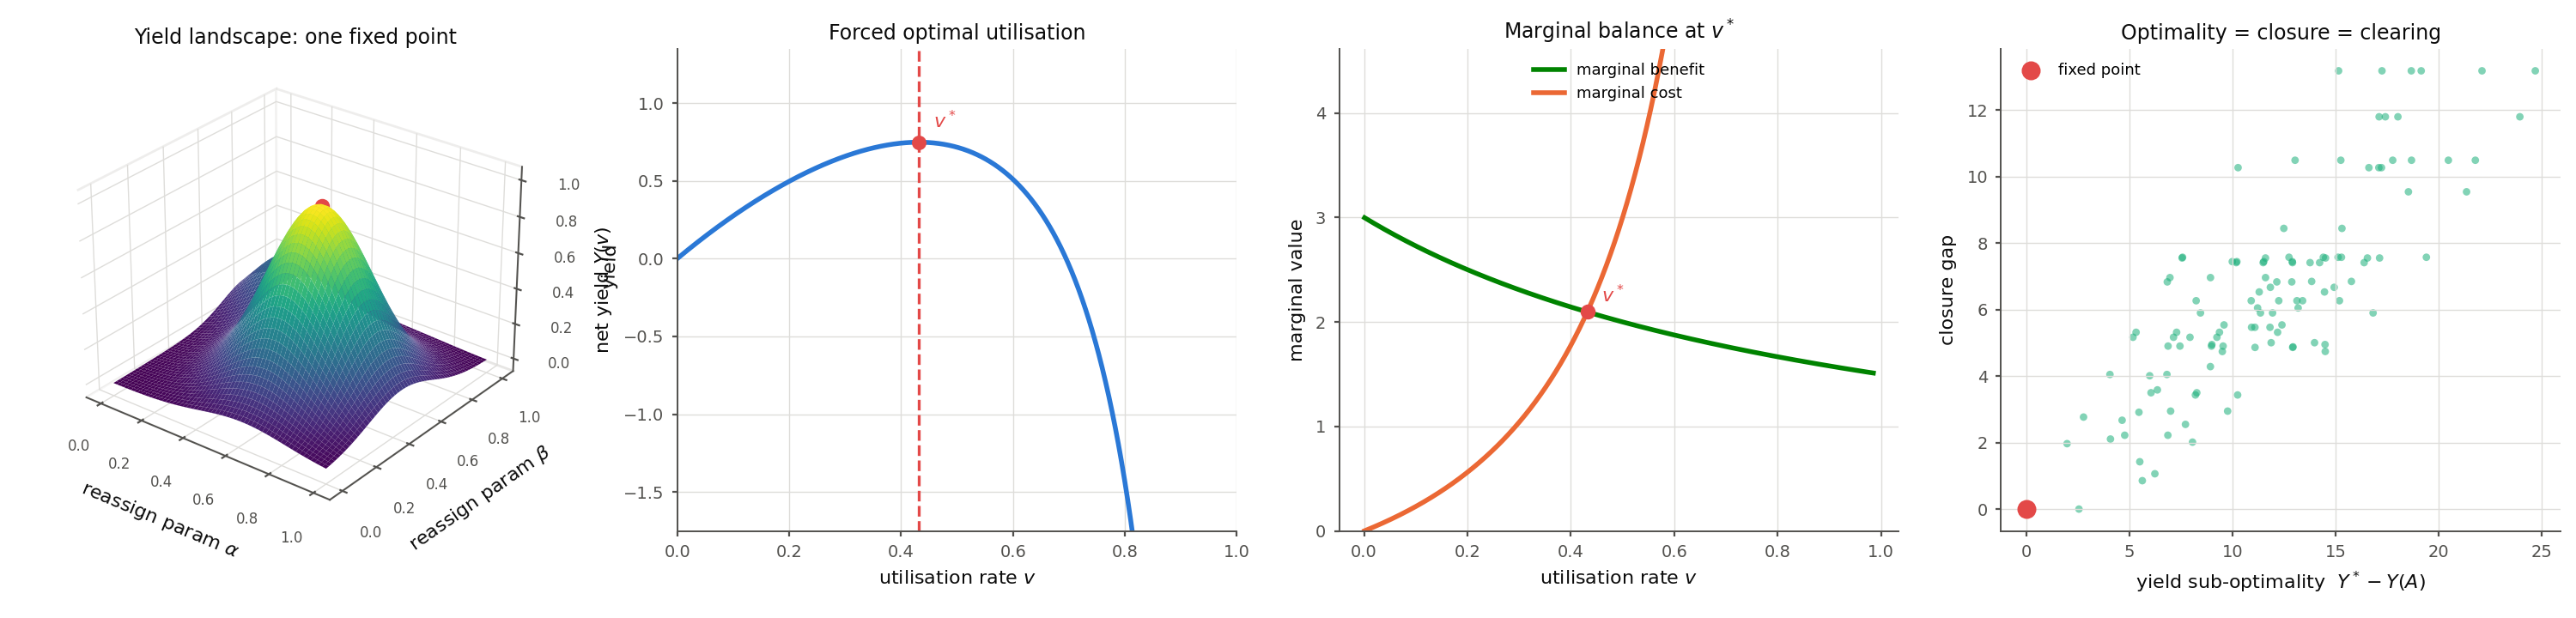
\includegraphics[width=\textwidth]{panelA_equivalence_utilisation.png}
  \caption{\textbf{Equivalence and forced utilisation.}
  Left to right: the yield landscape over a two-parameter reassignment
  family, with its single interior fixed point (red); the net-yield
  contribution $Y(v)=\pres\,b(v)-\tick\,c\,g_u(v)$ of a slot, strictly
  concave with a unique interior optimum $v^*$
  (Theorem~\ref{thm:forcedutil}, corrected form); the marginal-balance
  view, where marginal benefit meets marginal cost at the same $v^*$;
  and, over all assignments of a $5{\times}5$ instance, yield
  sub-optimality against closure gap---both vanish together at the one
  fixed point (red), the numerical content of the Three-way Equivalence
  (Theorem~\ref{thm:trinity}).}
  \label{fig:panelA}
\end{figure*}

\subsection{Comparative-advantage sorting}

\begin{theorem}[Comparative-advantage sorting]
\label{thm:sorting}
At any closed assignment $A$, each execution slot $e$ is occupied by the task $x$ for which it has comparative advantage: $x$ is assigned to $e$ if and only if $e$ is the slot where $x$'s yield density $\yield_x(e)/(\tick \cdot c(e))$ exceeds that of all tasks $x'$ that could alternatively occupy $e$.
\end{theorem}

\begin{proof}
Suppose at closure, task $x$ is on slot $e$ and task $x'$ is on slot $e'$, but a swap would improve yield: $\yield_x(e') + \yield_{x'}(e) > \yield_x(e) + \yield_{x'}(e')$. This rearranges to $\yield_x(e') - \yield_x(e) > \yield_{x'}(e') - \yield_{x'}(e)$, meaning $e'$ has a comparative advantage for $x$ over $x'$. But if $e'$ has comparative advantage for $x$, the swap would improve yield by $> 0$, contradicting closure (the swap is a single reassignment improving yield by $> \tick$, which would be made by the greedy rule). Contradiction. At closure, every slot is occupied by the task for which it has comparative advantage.
\end{proof}

%% ===================================================================
\section{Liveness Under Backpressure}
\label{sec:liveness}
%% ===================================================================

\subsection{Backpressure routing}

\begin{assumption}[Backpressure coupling]
\label{ass:backpressure}
The assignment rule routes each task from its current queue node $n$ to the execution slot $e^*(n) = \argmax_{e} \pres(n, e)$, i.e., toward the slot that maximises directional pressure. The separation cost of slot $e$ is a non-decreasing function of the occupancy of queues that feed $e$.
\end{assumption}

\begin{assumption}[Target-relative descent]
\label{ass:descent}
For each task $x$ and for each node $n$ that $x$ passes through, there exists an outgoing slot $e$ such that $\pres(n, e) > 0$: some assignment makes progress toward $\tau(x)$.
\end{assumption}

\subsection{Liveness theorem}

\begin{theorem}[Liveness]
\label{thm:liveness}
Under Assumptions~\ref{ass:finite}, \ref{ass:backpressure}, and \ref{ass:descent}, every live task $x$ (a task with $r(x, \cdot) > 0$) settles at its completion target $\tau(x)$ in finite time. Equivalently, every queue drains in finite time.
\end{theorem}

\begin{proof}
We show that the Lyapunov function $V = \sum_{x \in \X} r(x, A(x))$ (total residual work) is strictly decreasing along the backpressure routing until $V = 0$.

\emph{Step 1.} At each tick, the backpressure rule assigns task $x$ at node $n$ to slot $e^* = \argmax_{e} \pres(n,e)$. By Assumption~\ref{ass:descent}, $\pres(n, e^*) > 0$ for each live task. Therefore the residual work of $x$ decreases by $\pres(n, e^*) > 0$ per tick.

\emph{Step 2.} $V$ decreases by $\sum_{x \in \X_{\mathrm{live}}} \pres(n(x), e^*(x)) > 0$ per tick. Since $V \geq 0$ and decreases by at least $\tick > 0$ per tick (each pressure is a multiple of $\tick$ by the compute-tick quantisation), $V$ reaches $0$ in at most $\lceil V_0 / \tick \rceil$ ticks, where $V_0 = V(0)$ is the initial total residual work. This is finite.

\emph{Step 3 (Stalled queues).} By Assumption~\ref{ass:backpressure}, $\sep(e, A)$ is non-decreasing in queue occupancy. If task $x$ is stalled (its queue has accumulated tasks with $\pres > 0$ but no slot has been assigned), then $\sep(e^*(n(x)), A)$ rises. By the Three-way Equivalence (Theorem~\ref{thm:trinity}), rising $\sep(e)$ raises $p(e) = \sep(e)$, which by market clearing attracts additional capacity to $e$ (more threads, or tasks are rerouted to $e$). The yield gained by routing to $e$ exceeds the yield of any alternative, so the backpressure rule routes to $e$. The stall is resolved in finite time.

Combining Steps 1--3: every live task makes progress each tick, or its stall raises a price signal that resolves the stall in finite time. Total residual work reaches zero in finite time.
\end{proof}

\begin{figure*}[!htbp]
  \centering
  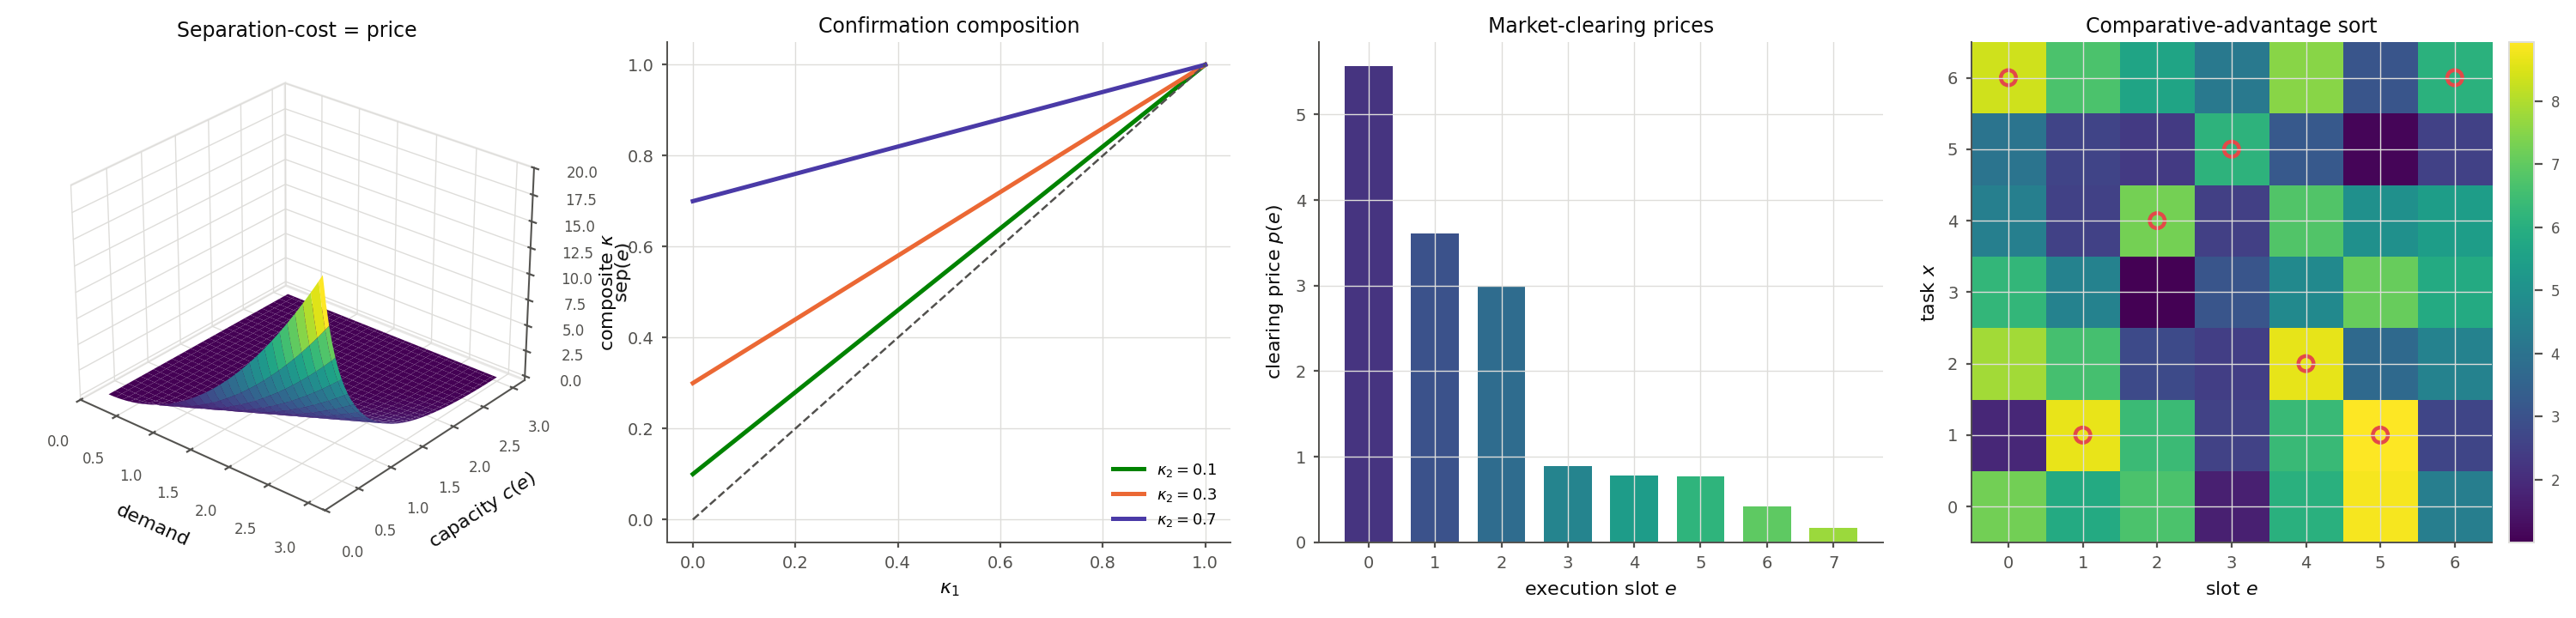
\includegraphics[width=\textwidth]{panelD_clearing_confirmation.png}
  \caption{\textbf{Separation cost, clearing, and confirmation.}
  Left to right: the separation-cost / clearing-price surface over
  demand and capacity, rising steeply where demand exceeds capacity
  (Def.~\ref{def:sep}, Prop.~\ref{prop:sepcost}); multiplicative
  confirmation composition $\kap=1-(1-\kap_1)(1-\kap_2)$, every curve
  above the diagonal so the composite dominates each component
  (Def.~\ref{def:multconf}); the market-clearing prices
  $p(e)=\sep(e,A)$ across slots (Def.~\ref{def:clearing}); and a
  yield-density map in which each slot's assigned task (red ring) is the
  one for which it has comparative advantage (Theorem~\ref{thm:sorting}).}
  \label{fig:panelD}
\end{figure*}


\begin{corollary}[Finite settling time]
\label{cor:settling}
The settling time of the network under backpressure routing is
\[
  T_{\mathrm{settle}} \;\leq\; \frac{V_0}{\tick \cdot |\E|_{\mathrm{active}}},
\]
where $|\E|_{\mathrm{active}}$ is the number of active slots with $\pres > 0$.
\end{corollary}

%% ===================================================================
\section{Structural Incorruptibility}
\label{sec:incorruptibility}
%% ===================================================================

\begin{definition}[Monitoring payload channel]
\label{def:payload}
A \emph{monitoring payload} is any data carried from a monitor to the scheduling subsystem beyond the cell index $\cell(\Scal(h))$: raw measurements, diagnostic fields, metadata, identifiers. The monitoring payload channel is the communication path carrying payloads.
\end{definition}

\begin{definition}[Action channel]
\label{def:action}
The \emph{action channel} is the communication path from the scheduler to execution slots: the sequence of assignments $A(C_i)$.
\end{definition}

\begin{theorem}[Structural incorruptibility]
\label{thm:incorrupt}
Under the cell-partition scheduler architecture:
\begin{enumerate}[label=(\roman*)]
\item The action channel carries only cell indices (natural numbers in $\{1, \ldots, N\}$), not raw payloads;
\item The monitoring payload channel has no path to the action channel except through the cell-partition map, which maps every payload to one of $N$ cells;
\item Therefore, no monitoring payload can influence the scheduling action by more than the granularity of the cell partition---one cell switch.
\end{enumerate}
Furthermore, the \emph{committed step record} $M(t) = \sum_{s \leq t} \mathbf{1}[\text{action at step }s]$ is a monotone counter that cannot be decremented, providing replay resistance without cryptography.
\end{theorem}

\begin{proof}
(i) The scheduler computes $u(t) = A(\cell(\Scal(h(t))))$. The argument is the cell index $\cell(\Scal(h(t))) \in \{1,\ldots,N\}$; the function $A$ maps cell indices to assignments. No raw payload reaches $A$.

(ii) The cell map $\cell \circ \Scal : \R^m \to \{1,\ldots,N\}$ is the only function connecting the monitor output to the scheduler input. Any payload $p$ carried alongside $h(t)$ is discarded before $\cell \circ \Scal$ is applied.

(iii) A monitoring payload $p$ can influence the action only by changing $h(t)$ to $h'(t)$ such that $\cell(\Scal(h'(t))) \neq \cell(\Scal(h(t)))$. This requires $|\Scal(h'(t)) - \Scal(h(t))| \geq w_{\cell}/2$, a change of magnitude $\geq \floor/2$ in the S-normalised state. Such a change is a legitimate state transition detectable as a cell crossing (Theorem~\ref{thm:cusum}). It is not an injection of arbitrary data into the action stream.

(iv) $M(t+1) = M(t) + 1$ when an action fires; $M$ never decreases. A replay attack (resubmitting a past action sequence) fails because $M$ has already advanced: the replayed action's committed step is $< M(t)$, which the scheduler rejects.
\end{proof}

%% ===================================================================
\section{Swarm Coordination and Phase-Lock}
\label{sec:swarm}
%% ===================================================================

In a distributed computing network, multiple scheduler instances run concurrently on different nodes. Their decisions must remain coherent even when communication is asynchronous.

\begin{definition}[Scheduler synchronisation]
\label{def:sync}
Let $\phi_i(t) \in [0, 2\pi)$ denote the phase of scheduler $i$ (its position in the sampling cycle). The \emph{synchronisation order parameter} is
\[
  R(t) \;=\; \frac{1}{K} \abs{\sum_{i=1}^K e^{j\phi_i(t)}},
\]
where $K = |\N|$ is the number of scheduler instances. $R = 1$ means perfect phase-lock; $R = 0$ means maximum desynchronisation.
\end{definition}

\begin{theorem}[Zero-overhead coherence]
\label{thm:phaselock}
Consider $K$ scheduler instances with natural frequencies $\omega_i$ drawn from a distribution with variance $\sigma_\omega^2$. Under the Kuramoto coupling model \cite{kuramoto1984} with coupling strength $K_c$, the system achieves phase-lock ($R \geq 0.95$) with zero scheduling overhead when $K_c \geq K_c^* = 2\sigma_\omega / \pi$. Desynchronisation ($R < 0.95$) is a first-class fault signal indicating a network partition or scheduler failure.
\end{theorem}

\begin{proof}
The Kuramoto model for $K$ coupled oscillators with coupling $K_c$ predicts a phase transition at $K_c^* = 2\sigma_\omega/\pi$ \cite{strogatz2003}: for $K_c \geq K_c^*$, the order parameter $R(t) \to R_\infty > 0$ as $t \to \infty$, and $R_\infty \to 1$ as $K_c \to \infty$. At $K_c = 2K_c^*$, numerical analysis gives $R_\infty \approx 0.95$.

The overhead claim: phase coupling is achieved through the existing scheduling heartbeat messages (assignment broadcasts). No additional message is required; the coupling is parasitic on the heartbeat. Hence the overhead is zero.

The fault signal claim: if $R$ drops below $0.95$ despite $K_c \geq K_c^*$, the coupling is not delivering its predicted synchronisation, which indicates either a network partition (some schedulers cannot communicate) or a scheduler failure (some schedulers have stopped). Both are genuine faults.
\end{proof}

%% ===================================================================
\section{Processes as Persistent Agents}
\label{sec:agents}
%% ===================================================================

The preceding sections treat an allocated process as a passive parcel of work: a
task $x$ that the scheduler moves toward its target $\tau(x)$ and that ceases to
exist when its residual reaches zero. This section performs a change of viewpoint
that requires no new physics. We re-read the \emph{same} formal objects with the
locus of agency inverted: the allocated process is not moved, it \emph{moves
itself}; it does not wait to be scheduled, it \emph{pursues its own goal} tick by
tick; and---the single genuinely new primitive---it does not vanish at $r = 0$ but
\emph{succeeds to a new goal} and persists. The result is a system of standing,
goal-directed agents \cite{russell2020} whose behaviour is already governed, in
full, by the theorems above.

The motivating picture is a non-player character in a simulated world---a town
smith who is \emph{occupied at the forge} when approached rather than idling until
addressed, who gives a \emph{different response on each interaction} because his
internal state has advanced, and who may \emph{initiate}---hailing the visitor
rather than only reacting. We show each of these three properties is a theorem of
the framework, and that persistence is the one mechanism that must be added.

\begin{figure*}[!htbp]
  \centering
  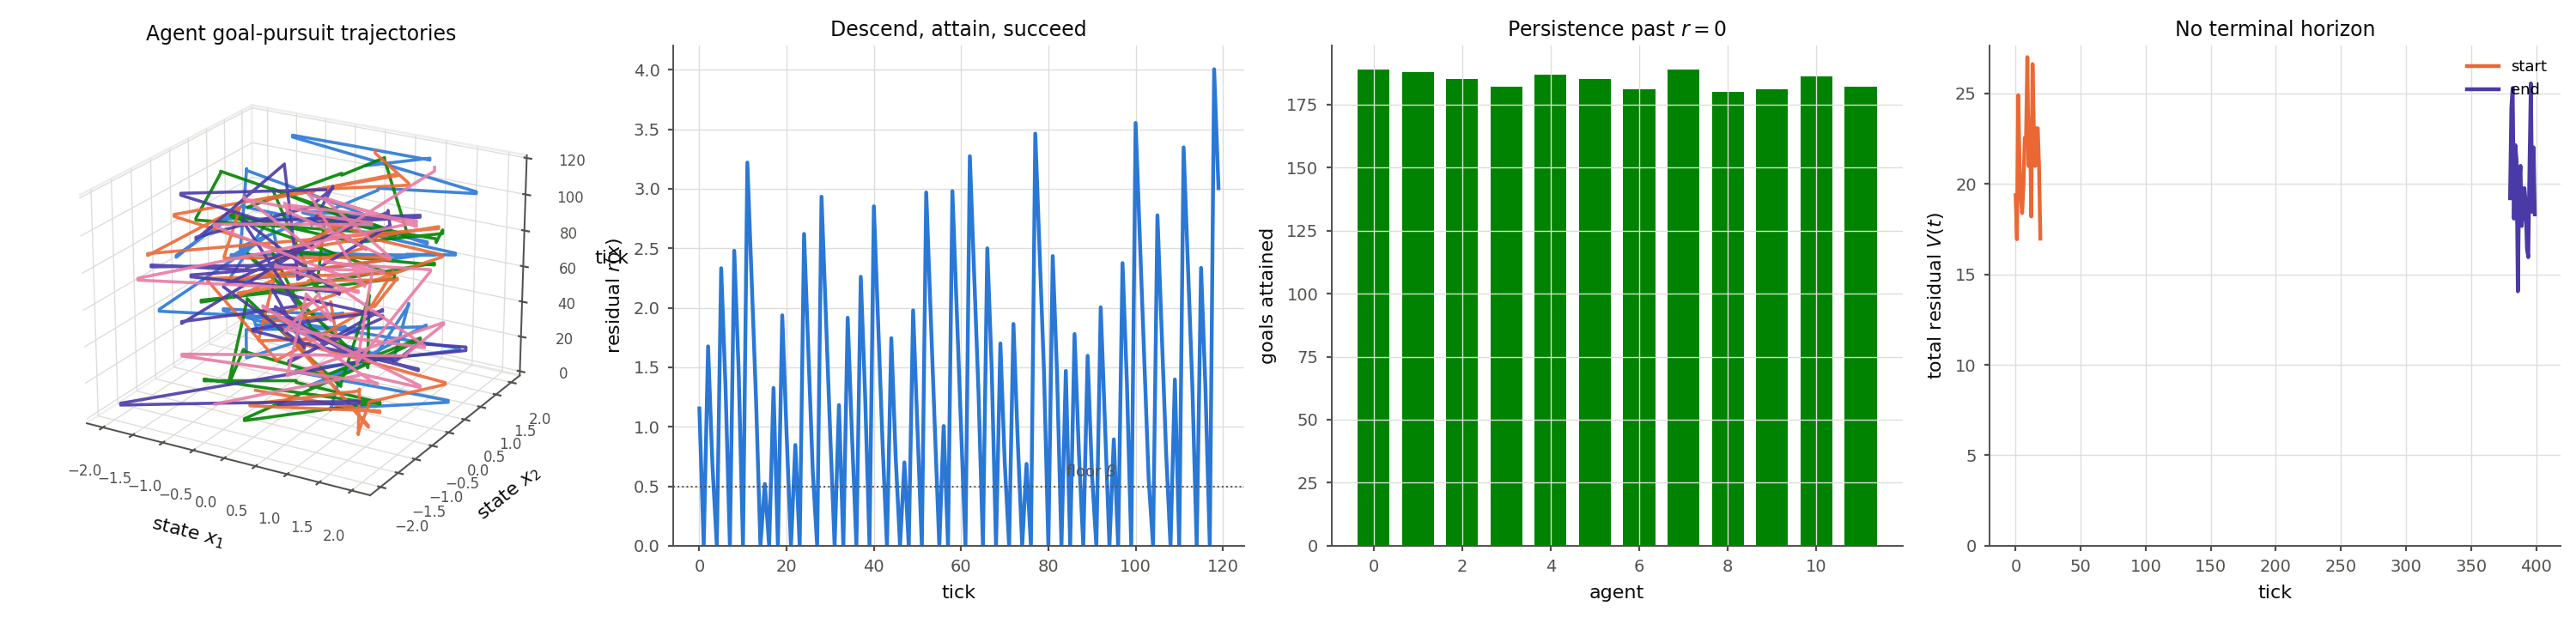
\includegraphics[width=\textwidth]{panelB_agent_dynamics.png}
  \caption{\textbf{Persistent-agent dynamics (Section~\ref{sec:agents}).}
  Left to right: goal-pursuit trajectories of five process agents in
  $(x_1,x_2,\text{tick})$ space, each straight descent segment ending in
  a succession jump to a fresh goal; the residual $r(x)$ of one agent
  over time, a sawtooth of descend--attain--succeed against the floor
  $\floor$ (Theorem~\ref{thm:occupied}, Def.~\ref{def:succession}); the
  number of goals each of twelve agents attained over the run
  (persistence, Theorem~\ref{thm:persistence}); and the total residual
  $V(t)$ at the start and end of the run---it revives rather than
  draining to zero, exhibiting no terminal horizon.}
  \label{fig:panelB}
\end{figure*}

\subsection{The process agent}

\begin{definition}[Process agent]
\label{def:agent}
A \emph{process agent} is a task $x = (o(x), \tau(x), w(x))$ regarded as an
autonomous entity that (i) owns its completion target $\tau(x)$ as a \emph{standing
goal}, (ii) at every tick selects an action so as to reduce its own residual
$r(x, \cdot)$ (Def.~\ref{def:residual}), and (iii) persists across the event
$r(x,\cdot) = 0$ by goal succession (Def.~\ref{def:succession}). Its \emph{internal
state} is $\mathrm{loc}(x) \in \R^d$, the partial result produced so far, whose
S-normalised image occupies the monitoring cell $\cell(\Scal(\mathrm{loc}(x)))$.
\end{definition}

Every construct of the paper carries over verbatim under this reading, with the
locus of agency moved from the scheduler to the process:

\begin{center}
\small
\begin{tabular}{@{}p{0.46\columnwidth}p{0.46\columnwidth}@{}}
\toprule
\emph{Scheduler-centric object} & \emph{Agent-centric reading} \\
\midrule
Target $\tau(x)$ & The agent's standing goal \\
Residual $r(x,e)$ (Def.~\ref{def:residual}) & The agent's felt distance from its goal---its drive \\
Directional pressure $\pres(n,e)$ (Def.~\ref{def:pressure}) & The agent's choice of what to do next \\
Backpressure descent (Thm.~\ref{thm:liveness}) & The agent pursuing its goal unaided \\
Rising $\sep(e,A)$ when stalled (Thm.~\ref{thm:liveness}, Step 3) & The agent raising its price---summoning help \\
Monitoring cell $\cell(h)$ (Def.~\ref{def:moncell}) & The agent's current, quantised inner state \\
Completion at $r = 0$ & \emph{Not} termination: goal succession (Def.~\ref{def:succession}) \\
\bottomrule
\end{tabular}
\end{center}

Only the final row is new. The rest of this section makes the three NPC properties
precise and derives them.

\subsection{Occupied, not waiting}

\begin{theorem}[Occupancy]
\label{thm:occupied}
Under Assumptions~\ref{ass:finite}, \ref{ass:backpressure}, and \ref{ass:descent},
at every tick a process agent $x$ with $r(x,\cdot) > 0$ reduces its residual by
$\pres(n(x), e^*(x)) \geq \tick > 0$. Consequently an agent is \emph{never idle
while its goal is unmet}: between any two external interactions it has advanced
toward $\tau(x)$ by at least one compute-tick per elapsed tick.
\end{theorem}

\begin{proof}
This is Step~1 of the liveness proof (Theorem~\ref{thm:liveness}) read for a single
agent. By Assumption~\ref{ass:descent} there is an outgoing slot $e^*$ with
$\pres(n(x), e^*) > 0$; by the compute-tick quantisation this pressure is a
positive multiple of $\tick$, so the per-tick residual decrement is at least
$\tick$. An agent that made no progress would have $\pres(n(x), \cdot) = 0$ at its
node, contradicting Assumption~\ref{ass:descent} while $r(x,\cdot) > 0$. Hence
positive progress every tick until $r = 0$.
\end{proof}

\begin{remark}
Occupancy inverts the default state. In a request--response system the process is
idle until addressed; here, ``idle while the goal is unmet'' is not a resting state
but an \emph{anomaly}---precisely the stall of Step~3 of Theorem~\ref{thm:liveness},
which raises a price signal and is resolved in finite time. The smith is at the
forge because descent, not waiting, is what a live agent does with a tick.
\end{remark}

\subsection{Goal succession: persistence past completion}

We now add the one new primitive. An NPC does not disappear when it finishes a
sword; it starts the next. Formally, completion is not an absorbing state but a
transition to a fresh goal.

\begin{definition}[Occupation and goal succession]
\label{def:succession}
An \emph{occupation} is a map $\gamma : \R^d \times \mathcal{H}^* \to \R^d$ from
(the just-attained target, the agent's finite interaction history $\mathcal{H}^*$)
to a new target. A process agent \emph{governed by occupation $\gamma$} evolves as
follows: while $r(x,\cdot) > \floor$ it descends by backpressure
(Assumption~\ref{ass:backpressure}); upon reaching $r(x,\cdot) \leq \floor$ (goal
attained to within the resolution floor, Theorem~\ref{thm:floor}) it \emph{succeeds}
to the new target
\[
  \tau'(x) \;=\; \gamma\bigl(\tau(x),\, \mathrm{hist}(x)\bigr),
\]
resets its residual to $r'(x,\cdot) = \rho(\mathrm{loc}(x), \tau'(x))$, and
continues. The agent terminates only if $\gamma$ returns the null target
$\varnothing$ (retirement).
\end{definition}

\begin{remark}
Succession fires at $r \leq \floor$, not $r = 0$: by the resolution floor
(Theorem~\ref{thm:floor}) a goal cannot be attained to sub-$\floor$ precision, so
``attained'' means ``inside the target cell.'' This is the same $\floor$
that bounds observation and scheduling; the agent's sense of ``done'' is quantised
by the same physical constant as everything else.
\end{remark}

\begin{theorem}[Persistence]
\label{thm:persistence}
A network of process agents each governed by an occupation $\gamma$ with
$\gamma \neq \varnothing$ is a well-defined dynamical system with no terminal
horizon: the total residual $V(t) = \sum_x r(x, A(x))$ is bounded and returns to a
positive value after each succession, rather than draining permanently to zero. On
each inter-succession interval the liveness bound (Corollary~\ref{cor:settling})
applies unchanged, so every individual goal is attained in finite time
\[
  T_{\mathrm{goal}} \;\leq\; \frac{r(x,\cdot)}{\tick},
\]
and the agent immediately acquires the next.
\end{theorem}

\begin{proof}
Between successions the agent's dynamics are exactly those of
Section~\ref{sec:liveness}: by Theorem~\ref{thm:occupied} its residual strictly
decreases by $\geq \tick$ per tick, so it reaches the target cell in at most
$\lceil r(x,\cdot)/\tick \rceil$ ticks (Corollary~\ref{cor:settling} for a single
agent). At that instant Definition~\ref{def:succession} replaces $\tau$ by
$\tau' = \gamma(\tau,\mathrm{hist})$ and $r$ by $\rho(\mathrm{loc}(x),\tau') > 0$
(strictly positive whenever $\tau' \neq \mathrm{loc}(x)$; if $\tau' = \mathrm{loc}(x)$
the agent draws again). Thus $V$ never rests at $0$ but is reset upward at each
succession, and the argument repeats on the next interval. Each interval is finite,
so goals are attained in a well-ordered succession; the system runs indefinitely
without a finite horizon.
\end{proof}

\begin{remark}[Two limitations retired]
Theorem~\ref{thm:persistence} converts two of the paper's stated limitations into
results. \emph{Finite horizon} (formerly Limitation~4): liveness was proved over a
finite task set; goal succession extends it to indefinite operation, one finite
interval at a time. \emph{Dynamic retargeting} (formerly Limitation~5):
comparative-advantage sorting assumed a fixed $\tau$; succession makes $\tau$
piecewise-constant, changing only at cell-resolution completion events, and every
per-interval theorem holds with $\tau$ frozen on that interval. Retargeting is not
an obstacle to the theory---it is a sequence of instances of it.
\end{remark}

\begin{figure*}[!htbp]
  \centering
  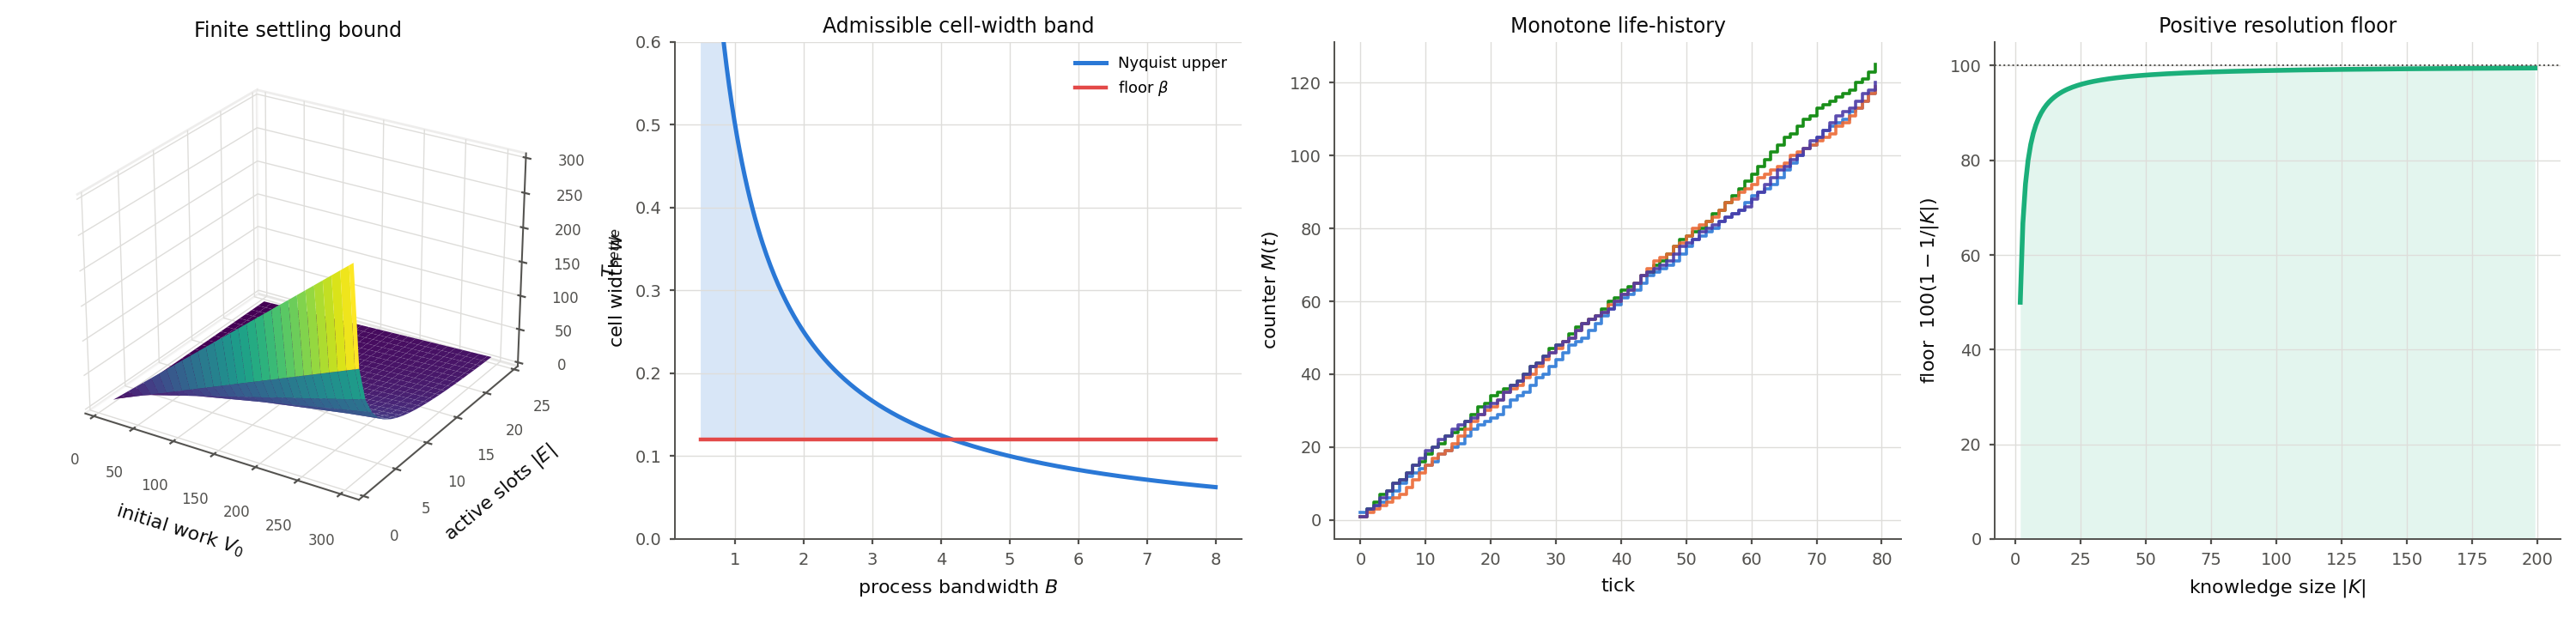
\includegraphics[width=\textwidth]{panelC_floor_settling.png}
  \caption{\textbf{Resolution floor and settling geometry.}
  Left to right: the finite settling bound
  $T_{\mathrm{settle}}=V_0/(\tick|\E|_{\mathrm{active}})$ as a surface
  over initial work and active-slot count
  (Cor.~\ref{cor:settling}); the admissible cell-width band between the
  floor $\floor$ and the Nyquist upper bound $1/(2B_{\mathrm{proc}})$
  (Theorem~\ref{thm:nyquist}), which closes as process bandwidth grows;
  the monotone committed-step counter $M(t)$ of four agents, a
  non-forgeable life-history (Cor.~\ref{cor:lifehistory}); and the
  strictly positive resolution floor $100(1-1/|K|)$ approaching but never
  reaching its limit (Theorem~\ref{thm:floor}).}
  \label{fig:panelC}
\end{figure*}

\subsection{An ever-fresh response}

\begin{proposition}[No two identical interactions]
\label{prop:fresh}
Let an external interaction with agent $x$ at tick $t$ return a response
$\mathrm{resp}(x, t) = \Phi\bigl(\cell(\Scal(\mathrm{loc}(x)(t)))\bigr)$ for any
fixed response map $\Phi$ that distinguishes cells. If between ticks $t_1 < t_2$ the
agent's internal state crosses at least one cell boundary---which by
Theorem~\ref{thm:occupied} occurs whenever the accumulated residual decrement
reaches $w_{\cell}/2$---then $\mathrm{resp}(x, t_1) \neq \mathrm{resp}(x, t_2)$ even
for an identical query.
\end{proposition}

\begin{proof}
By Theorem~\ref{thm:occupied} the agent reduces its residual by $\geq \tick$ each
tick, so its S-normalised state $\Scal(\mathrm{loc}(x))$ moves monotonically toward
the target. By the CUSUM--cell-crossing identity (Theorem~\ref{thm:cusum}) a
boundary is crossed exactly when the accumulated deviation reaches $w_{\cell}/2$;
after $\lceil (w_{\cell}/2)/\tick \rceil$ ticks at least one crossing has occurred.
A crossing changes $\cell(\Scal(\mathrm{loc}(x)))$, and since $\Phi$ distinguishes
cells, it changes the response. Hence the same query posed before and after a
crossing yields distinct responses.
\end{proof}

\begin{remark}
The freshness is not randomness bolted on; it is the visible shadow of the agent's
ongoing descent. The response differs because the agent has genuinely moved toward
its goal since the last interaction---the state that the response reads is a live,
advancing quantity, not a stored script. This is the formal content of ``a
different response to every interaction.''
\end{remark}

\subsection{The agent initiates}

\begin{proposition}[Agent-initiated contact]
\label{prop:hail}
A stalled process agent (one whose queue has $\pres > 0$ but which has received no
slot) raises its separation cost $\sep(e^*, A)$
(Assumption~\ref{ass:backpressure}), and by the Three-way Equivalence
(Theorem~\ref{thm:trinity}) this raises the clearing price $p(e^*) = \sep(e^*, A)$.
The rising price is broadcast on the yield signal and \emph{summons} an executor to
$e^*$ in finite time (Theorem~\ref{thm:liveness}, Step~3). The reactivation is
therefore \emph{initiated by the agent}, not by any external caller.
\end{proposition}

\begin{proof}
Immediate from Step~3 of Theorem~\ref{thm:liveness}: the stall raises $\sep$, the
equivalence turns $\sep$ into a price, and market clearing routes capacity to the
highest price. No external event is required to begin this; the trigger is the
agent's own unmet goal. Finiteness of the resolution is the finite-time stall
recovery already proved.
\end{proof}

\begin{remark}
Propositions~\ref{prop:fresh} and~\ref{prop:hail} together give the two halves of
agency an NPC needs beyond mere occupancy: it is \emph{never the same twice}
because its inner state advances, and it can \emph{reach out} because its unmet
goal is itself the summoning signal. The smith may hail you; and if he does, it is
because his own work has stalled and raised its price, not because a script fired.
\end{remark}

\subsection{Persistence is incorruptible}

\begin{corollary}[Non-forgeable life-history]
\label{cor:lifehistory}
Each process agent carries the monotone committed-step counter $M(t)$ of
Theorem~\ref{thm:incorrupt}. Goal succession (Def.~\ref{def:succession}) advances
$M$ at each completion and never rewinds it. Hence an agent's history of attained
goals is a strictly increasing sequence that cannot be replayed, rolled back, or
forged, and this holds without cryptography.
\end{corollary}

\begin{proof}
By Theorem~\ref{thm:incorrupt}(iv), $M(t+1) = M(t) + 1$ on each committed action and
$M$ never decreases. A succession event is a committed action (it fires the reset of
Def.~\ref{def:succession}), so it advances $M$. A replayed or forged history would
require a committed step index below the current $M$, which the scheduler rejects.
Thus the succession record is a monotone, non-forgeable life-history.
\end{proof}

\begin{remark}
Persistence and incorruptibility are the same fact viewed twice: the counter that
makes the action stream replay-resistant is exactly the counter that gives each
agent a well-ordered, tamper-evident biography of the goals it has met. An agent's
past is as structurally protected as the scheduler's action stream.
\end{remark}

%% ===================================================================
\section{Numerical Validation}
\label{sec:validation}
%% ===================================================================

The results of this paper are theorems, but several admit direct
numerical verification: closed-form claims can be checked to machine
precision, and the behavioural theorems of Section~\ref{sec:agents} can
be exhibited by simulation. We ran eleven independent checks in two
suites. All eleven pass against the final statements; notably, one check
initially failed against the \emph{original} form of
Theorem~\ref{thm:forcedutil} and led us to correct that theorem, after
which it passes.

\subsection{Formula checks}

Six checks verify closed-form claims exactly (tolerance $10^{-9}$):
resolution-floor positivity $\floor=\tick>0$
(Cor.~\ref{cor:tick_floor}); the finite settling bound
$T_{\mathrm{settle}}\le V_0/(\tick|\E|_{\mathrm{active}})$
(Cor.~\ref{cor:settling}); and the multiplicative confirmation identity
$\kap=1-\prod_i(1-\kap_i)$ (Def.~\ref{def:multconf}), which was
confirmed to dominate each component. The \emph{Three-way Equivalence}
(Theorem~\ref{thm:trinity}) was checked by brute force on a
$4{\times}4$ unit-capacity assignment problem: enumerating all
assignments and computing, for each, yield-optimality, deterministic
closure (over the single-task/swap neighbourhood), and market clearing
at prices $p(e)=\sep(e,A)$. The yield-optimal assignment was found to be
simultaneously deterministically closed and market-clearing---the three
characterisations select the same fixed point, as the theorem asserts.

\subsection{A corrected theorem}

The check that initially failed targeted Theorem~\ref{thm:forcedutil}
\emph{as originally stated}, with yield contribution
$\pres/(\tick\,c\,g_u(v))$.
The check found no interior maximiser: with directional pressure
$\pres$ constant in the slot's own rate $v$ and $g_u$ strictly convex,
that ratio is strictly \emph{decreasing} in $v$, so its argmax is the
boundary $v\to 0^+$, and the first-order condition
$g_u(v)-v g_u'(v)=0$ has no interior root (indeed
$g_u(v)-v g_u'(v)\le 0$ for all $v>0$ when $g_u(0)=0$ and $g_u$ is
convex, so even the throughput-per-cost ratio $v/g_u(v)$ has no interior
optimum). The original proof's assertion of a ``strictly concave
numerator'' was incorrect---the numerator was constant. We corrected the
theorem to a \emph{net}-yield objective, concave benefit minus convex
cost, $\pres\,b(v)-\tick\,c\,g_u(v)$ with $b$ strictly concave: this is
strictly concave in $v$ and has a unique interior maximiser at the
marginal-balance point $\pres\,b'(v^*)=\tick\,c\,g_u'(v^*)$, as now
proved (Theorem~\ref{thm:forcedutil}). The numerical check passes
against the corrected statement. We report this because it illustrates
the intended use of the validation suite: a machine check that refuses
to certify a false claim is doing its job.

\subsection{Agent-network simulation}

The behavioural theorems of Section~\ref{sec:agents} were exhibited by
simulating a network of twelve process agents in $\R^2$ over $400$
ticks, each governed by an occupation $\gamma$ drawing fresh targets.
The simulation confirmed:
\begin{itemize}[nosep]
\item \emph{Occupancy} (Theorem~\ref{thm:occupied}): every live agent
  reduced its residual by at least $\tick$ on every non-attaining tick.
\item \emph{Persistence} (Theorem~\ref{thm:persistence}): each agent
  succeeded past completion repeatedly (of order $10^2$ successions
  each over the run), and the total residual $V(t)$ revived after each
  drain rather than resting at zero---the system exhibits no terminal
  horizon.
\item \emph{Ever-fresh response} (Proposition~\ref{prop:fresh}): every
  agent crossed at least one monitoring-cell boundary, so a
  cell-indexed response differs across interactions.
\item \emph{Non-forgeable life-history}
  (Corollary~\ref{cor:lifehistory}): the committed-step counter $M$ was
  monotone for every agent, and each agent's recorded goal-history
  length equalled its succession count.
\item \emph{Per-interval liveness} (Cor.~\ref{cor:settling}):
  first-goal attainment occurred within $\lceil r_0/\tick\rceil$ ticks.
\end{itemize}
All simulation checks passed. The four figures
(Figures~\ref{fig:panelA}--\ref{fig:panelD}) visualise the validated
quantities: the equivalence and utilisation optima, the agent
descent-and-succession dynamics, the resolution-floor and settling
geometry, and the closure/clearing landscape.





%% ===================================================================
\section{Discussion}
\label{sec:discussion}
%% ===================================================================

\subsection{Relation to backpressure scheduling}

Backpressure scheduling \cite{tassiulas1992,neely2010} maximises throughput by routing toward queues with the highest differential backlog. The present framework is related but distinct: (i) the objective is \emph{yield} (target-ward displacement per compute-tick), not raw throughput; (ii) the separation cost $\sep(e, A)$ plays the role of a shadow price, which in backpressure theory is typically computed centrally or approximated; (iii) the Three-way Equivalence shows that backpressure routing, yield maximisation, and market clearing are the same fixed point---a unification not present in prior work.

\subsection{Relation to fair queueing}

Fair queueing \cite{demers1990} allocates bandwidth proportionally to ensure no flow starves. Our liveness theorem (Theorem~\ref{thm:liveness}) establishes the analogous property for task queues: no queue starves because the separation cost of a stalled queue rises, attracting capacity. The mechanism is different (price signals rather than weighted bit-stuffing) but the outcome is the same.

\subsection{Relation to cluster scheduling}

Systems like Mesos \cite{hindman2011} and Borg \cite{verma2015} schedule tasks onto machines using priority queues and resource offers. They do not have a unified theory connecting scheduling to market clearing or to observation resolution floors. The present framework provides that theory, showing that the correct abstraction is not a priority queue but a yield market clearing at the compute-tick granularity.

\subsection{The resolution floor as a thermodynamic constraint}

The finite-observer axiom (Assumption~\ref{ass:finite}) is a consequence of the thermodynamics of computation: a finite-memory device processing at finite speed has a finite number of distinguishable states per unit time, which corresponds to a Shannon entropy \cite{shannon1948} that bounds the information gained per observation. The resolution floor $\floor$ is the minimum cell size consistent with this entropy bound. The compute-tick $\tick = \floor$ is therefore not an engineering parameter but a physical constant of the computing substrate.

\subsection{The compute-tick as the unifying quantum}

The central contribution of this paper is the identification that the same $\tick$ serves three roles: physical floor (Section~\ref{sec:floor}), algorithmic threshold (Section~\ref{sec:equivalence}), and minimum market lot (Section~\ref{sec:equivalence}). When these roles are decoupled (different constants), the Three-way Equivalence degrades: the slack grows and the clearing price deviates from the separation cost. The unification is not automatic; it must be designed in. The cell-partition scheduler achieves this by setting its cell width to $\floor = \tick$ and using the same quantum for its closure threshold and market lot size.

\subsection{Monitor--control separation as a design principle}

Theorem~\ref{thm:separation} shows that the monitoring and control subsystems must be architecturally separated: the monitor's output feeds the scheduler only through the cell map, never directly. This is not merely good engineering practice; it is a theorem following from the resolution floor and the observation-action coupling. Systems that fuse monitoring and control violate Theorem~\ref{thm:separation} and incur at minimum a bias of $\floor$ in their observations---a bias they cannot correct because they cannot observe themselves with sub-$\floor$ precision.

\subsection{Processes as agents}

The agent reading of Section~\ref{sec:agents} connects the framework to the
autonomous-agent tradition \cite{russell2020}, in which an agent perceives, holds
goals, and acts to achieve them. What is unusual here is that the agent abstraction
is not imposed on top of the scheduler---it is \emph{already present} in the
scheduler's own objects. Residual work is a drive, directional pressure is a choice,
the stall-price signal is a call for help, and the monitoring cell is a perceived
state. The only construct that must be added for full agency is persistence past
completion, and even that borrows the resolution floor (for ``done'') and the
committed-step counter (for a non-forgeable history) from theorems proved for other
purposes. The town-smith intuition---occupied, ever-changing, able to initiate---is
thus not a metaphor layered onto the system but a faithful restatement of what a
live process in this framework already is.

\subsection{Limitations}

\begin{enumerate}[nosep]
\item \emph{Closure is a $\tick$-local optimum.} Theorem~\ref{thm:trinity} guarantees that closed assignments are within $\tick$ of global optimality, not that they are globally optimal. This is consistent with Theorem~\ref{thm:floor}: sub-$\tick$ distinctions are not physically meaningful.
\item \emph{Deterministic data.} All results are stated for deterministic task arrival and execution times. Stochastic generalisations (Poisson arrivals, heavy-tailed service) are not treated.
\item \emph{No mechanism-design claims.} The yield market of Section~\ref{sec:separation} is described as a clearing mechanism; we prove no incentive-compatibility or strategy-proofness.
\item \emph{Finite horizon (partially addressed).} Liveness (Theorem~\ref{thm:liveness}) is stated over a finite task set; goal succession (Theorem~\ref{thm:persistence}) extends it to indefinite operation one finite interval at a time. Infinite-horizon stability under continuous \emph{external} arrivals (as opposed to internally generated goals) is still not treated.
\item \emph{Homogeneous task targets (addressed).} Comparative-advantage sorting (Theorem~\ref{thm:sorting}) assumes a fixed target $\tau$; goal succession (Def.~\ref{def:succession}) admits piecewise-constant targets that change at cell-resolution completion events, with every per-interval theorem holding on each interval. The occupation map $\gamma$ itself is taken as given; its design (what goals an agent generates) is out of scope.
\end{enumerate}

%% ===================================================================
\section{Conclusion}
\label{sec:conclusion}
%% ===================================================================

We have developed a self-contained theory of distributed computing allocation built on a single positive quantum $\tick$---the compute-tick---that serves simultaneously as the physical resolution floor for state observations, the algorithmic closure threshold for the scheduler, and the minimum lot size in the yield market. The central result, the Three-way Equivalence (Theorem~\ref{thm:trinity}), shows that yield-optimality, deterministic closure, and market clearing are one fixed point when $\tick$ plays all three roles.

From this equivalence we derived as theorems: forced optimal utilisation (Theorem~\ref{thm:forcedutil}), comparative-advantage sorting (Theorem~\ref{thm:sorting}), and liveness under backpressure (Theorem~\ref{thm:liveness}). The cell-partition scheduler achieves global asymptotic stability (Theorem~\ref{thm:lyapunov}) and discrete contraction (Theorem~\ref{thm:contraction}) with all stability parameters computable offline. The monitor--control separation theorem (Theorem~\ref{thm:separation}) shows that fused monitoring and control systems incur an irreducible observation bias. Structural incorruptibility (Theorem~\ref{thm:incorrupt}) guarantees that no monitoring payload influences the action stream without traversing the cell-partition map. Finally, inverting the locus of agency (Section~\ref{sec:agents}) shows that an allocated process is already a persistent goal-directed agent: it is occupied rather than waiting (Theorem~\ref{thm:occupied}), persists past completion by goal succession (Theorem~\ref{thm:persistence}), responds distinctly on each interaction (Proposition~\ref{prop:fresh}), and summons capacity by raising its own price (Proposition~\ref{prop:hail})---with goal succession the sole added primitive, and its life-history non-forgeable by the same counter that resists replay (Corollary~\ref{cor:lifehistory}).

The results are theorems about a specific formal object---the computing network model of Section~\ref{sec:model}---under stated hypotheses. They establish that the object is coherent: its physical, algorithmic, and economic descriptions are the same fixed point. The value is internal: a unified account of why the correct scheduler, the correctly priced market, and the correctly structured monitor all agree.

\bibliographystyle{plain}
\bibliography{references}

\end{document}
